\hypertarget{application-to-data}{%
\section{\texorpdfstring{Application to
\cite{doreRelativeEffectsAnthropogenic2021}
data}{Application to  data}}\label{application-to-data}}

\label{sec:application-to-dorerelativeeffectsanthropogenic2021-data}

Here we apply the network clustering procedure (we refer to it as
\emph{netclustering}) to the data from
\cite{doreRelativeEffectsAnthropogenic2021}. These data are
plant-pollinator bipartite networks from differents areas and times.

In a second part we will use additional information for the networks to
try to identify the impact and correlations with the observed
structures.

\hypertarget{netclustering-with-the-iidtext-colbisbm-model}{%
\subsection{\texorpdfstring{Netclustering with the
\(iid\text{-}colBiSBM\)
model}{Netclustering with the iid\textbackslash text\{-\}colBiSBM model}}\label{netclustering-with-the-iidtext-colbisbm-model}}

We obtained the more interpretable results with \(iid\text{-}colBiSBM\)
model. This resulted in 5 collections to partition the \(M = 123\)
networks.

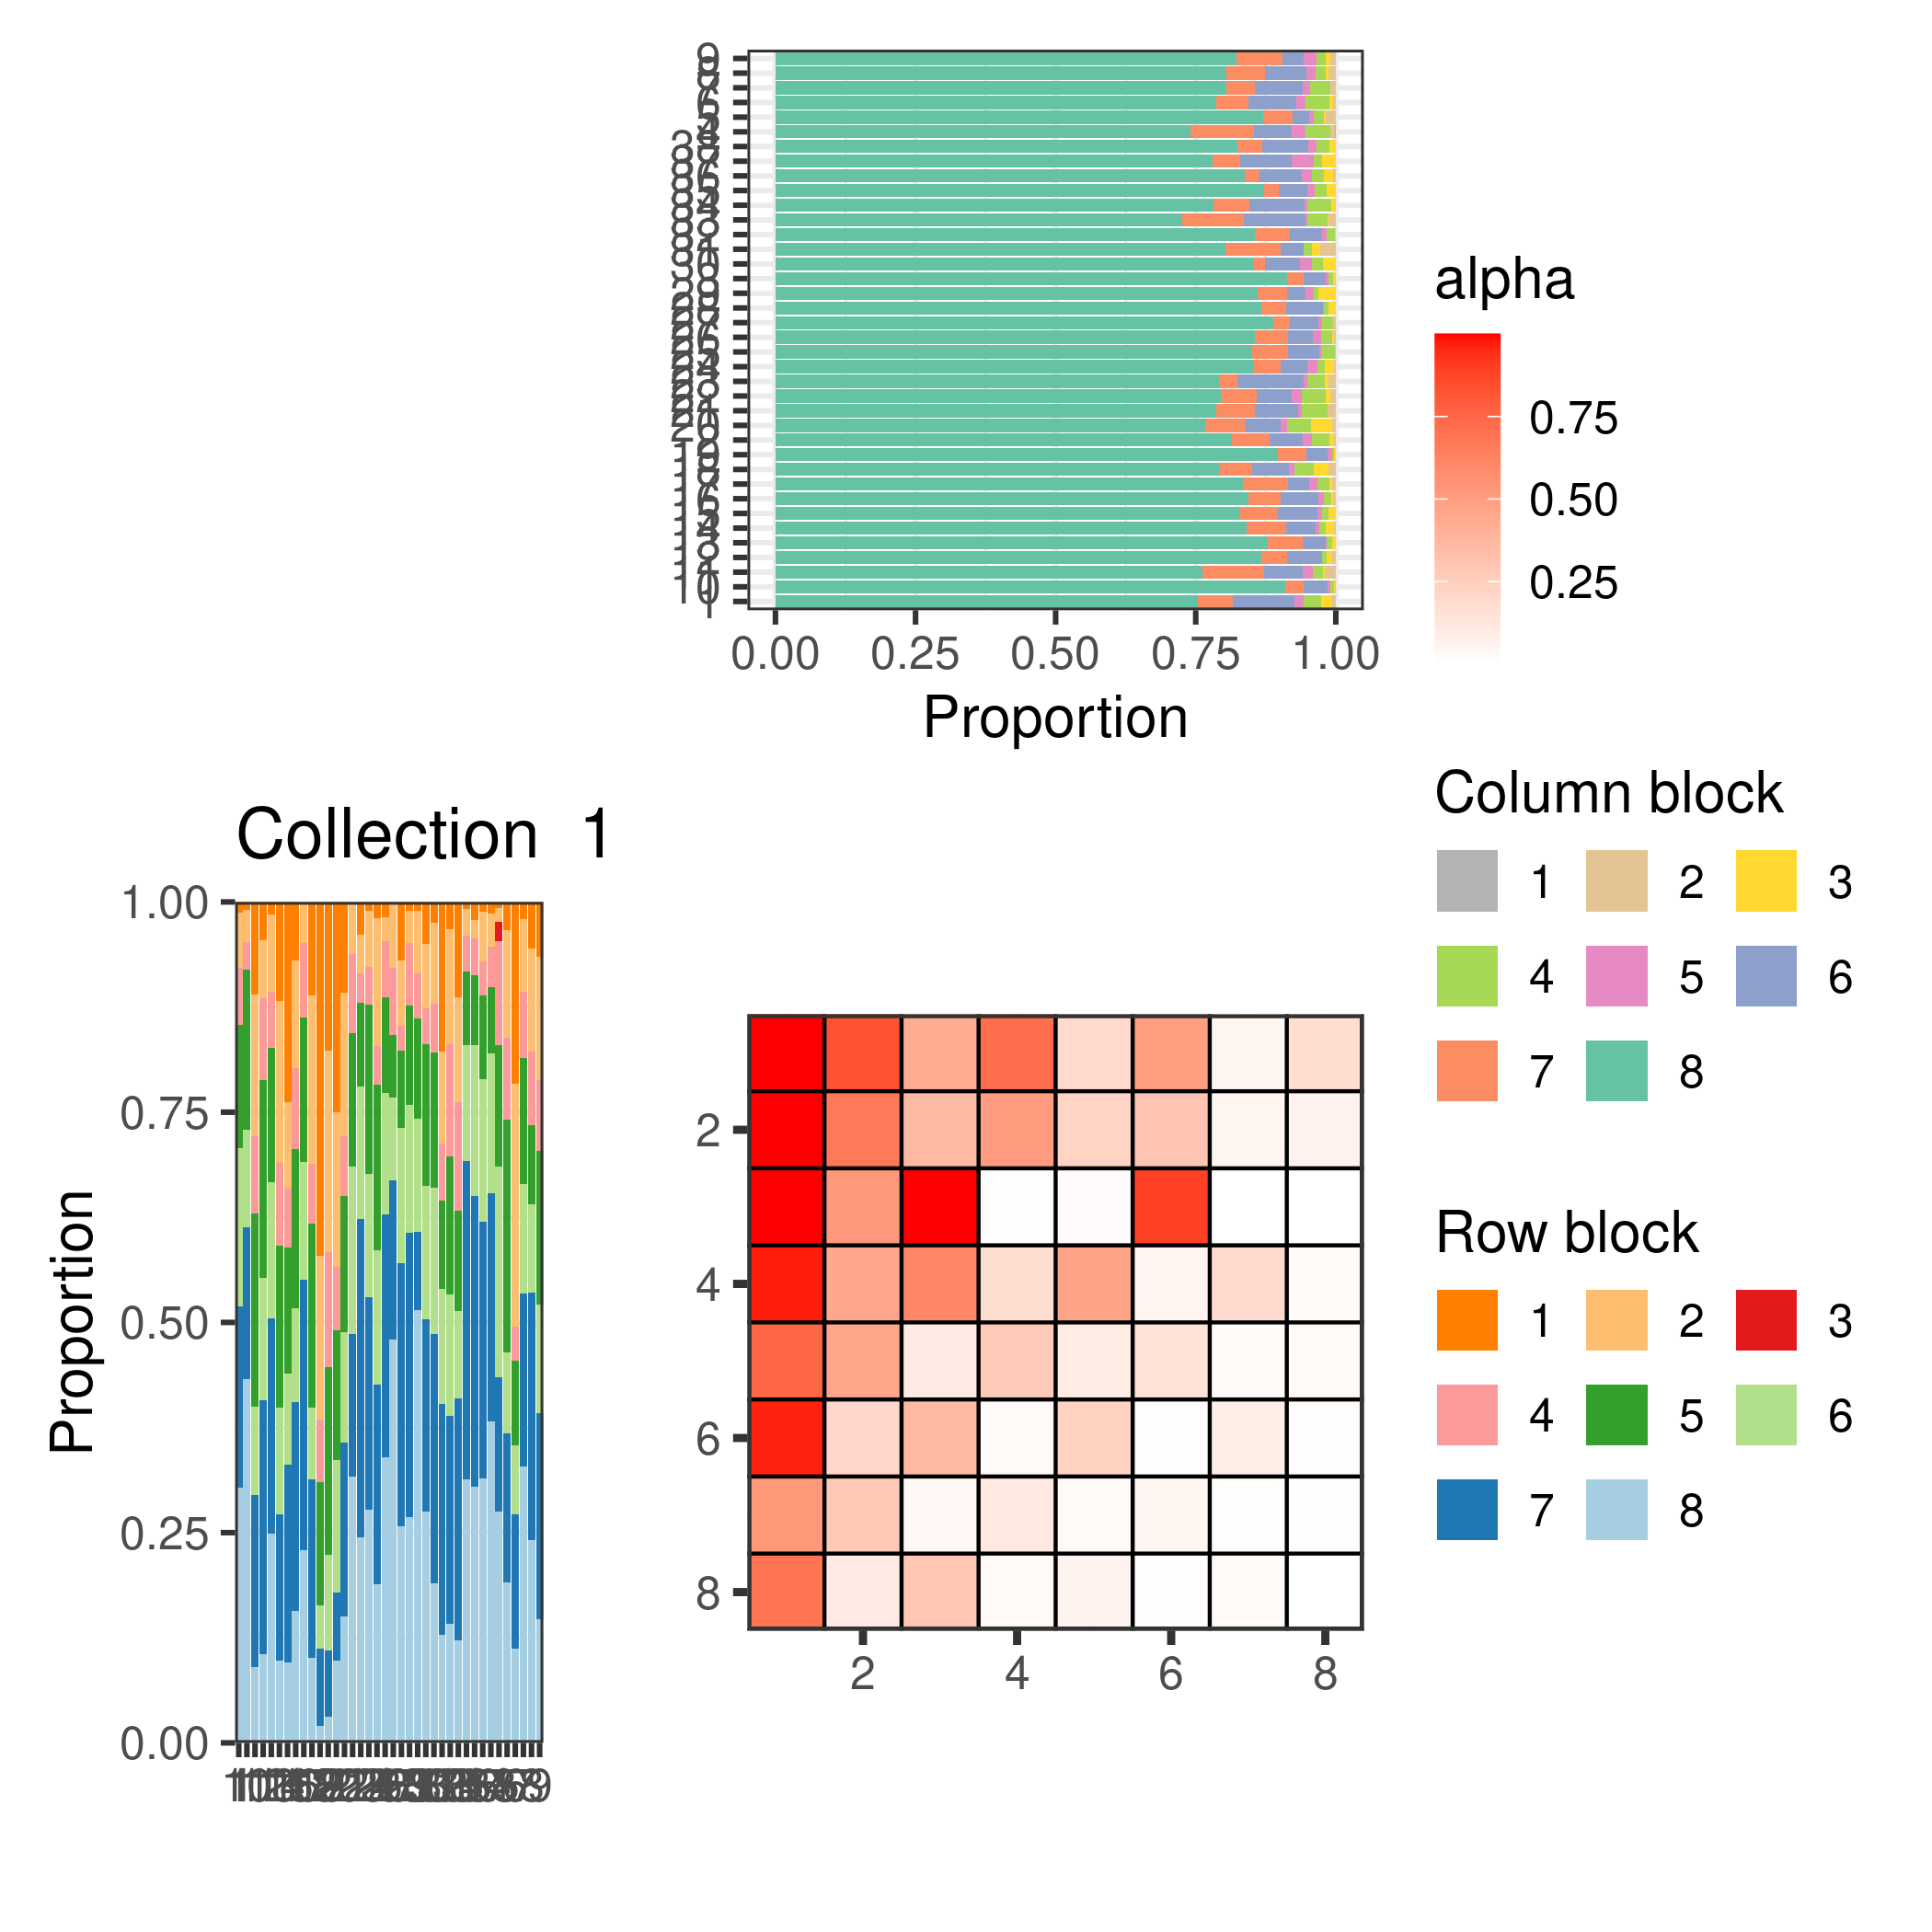
\includegraphics{./img/22d3409f045c956ffc0773e508871c61db4ad1e9.png}\newline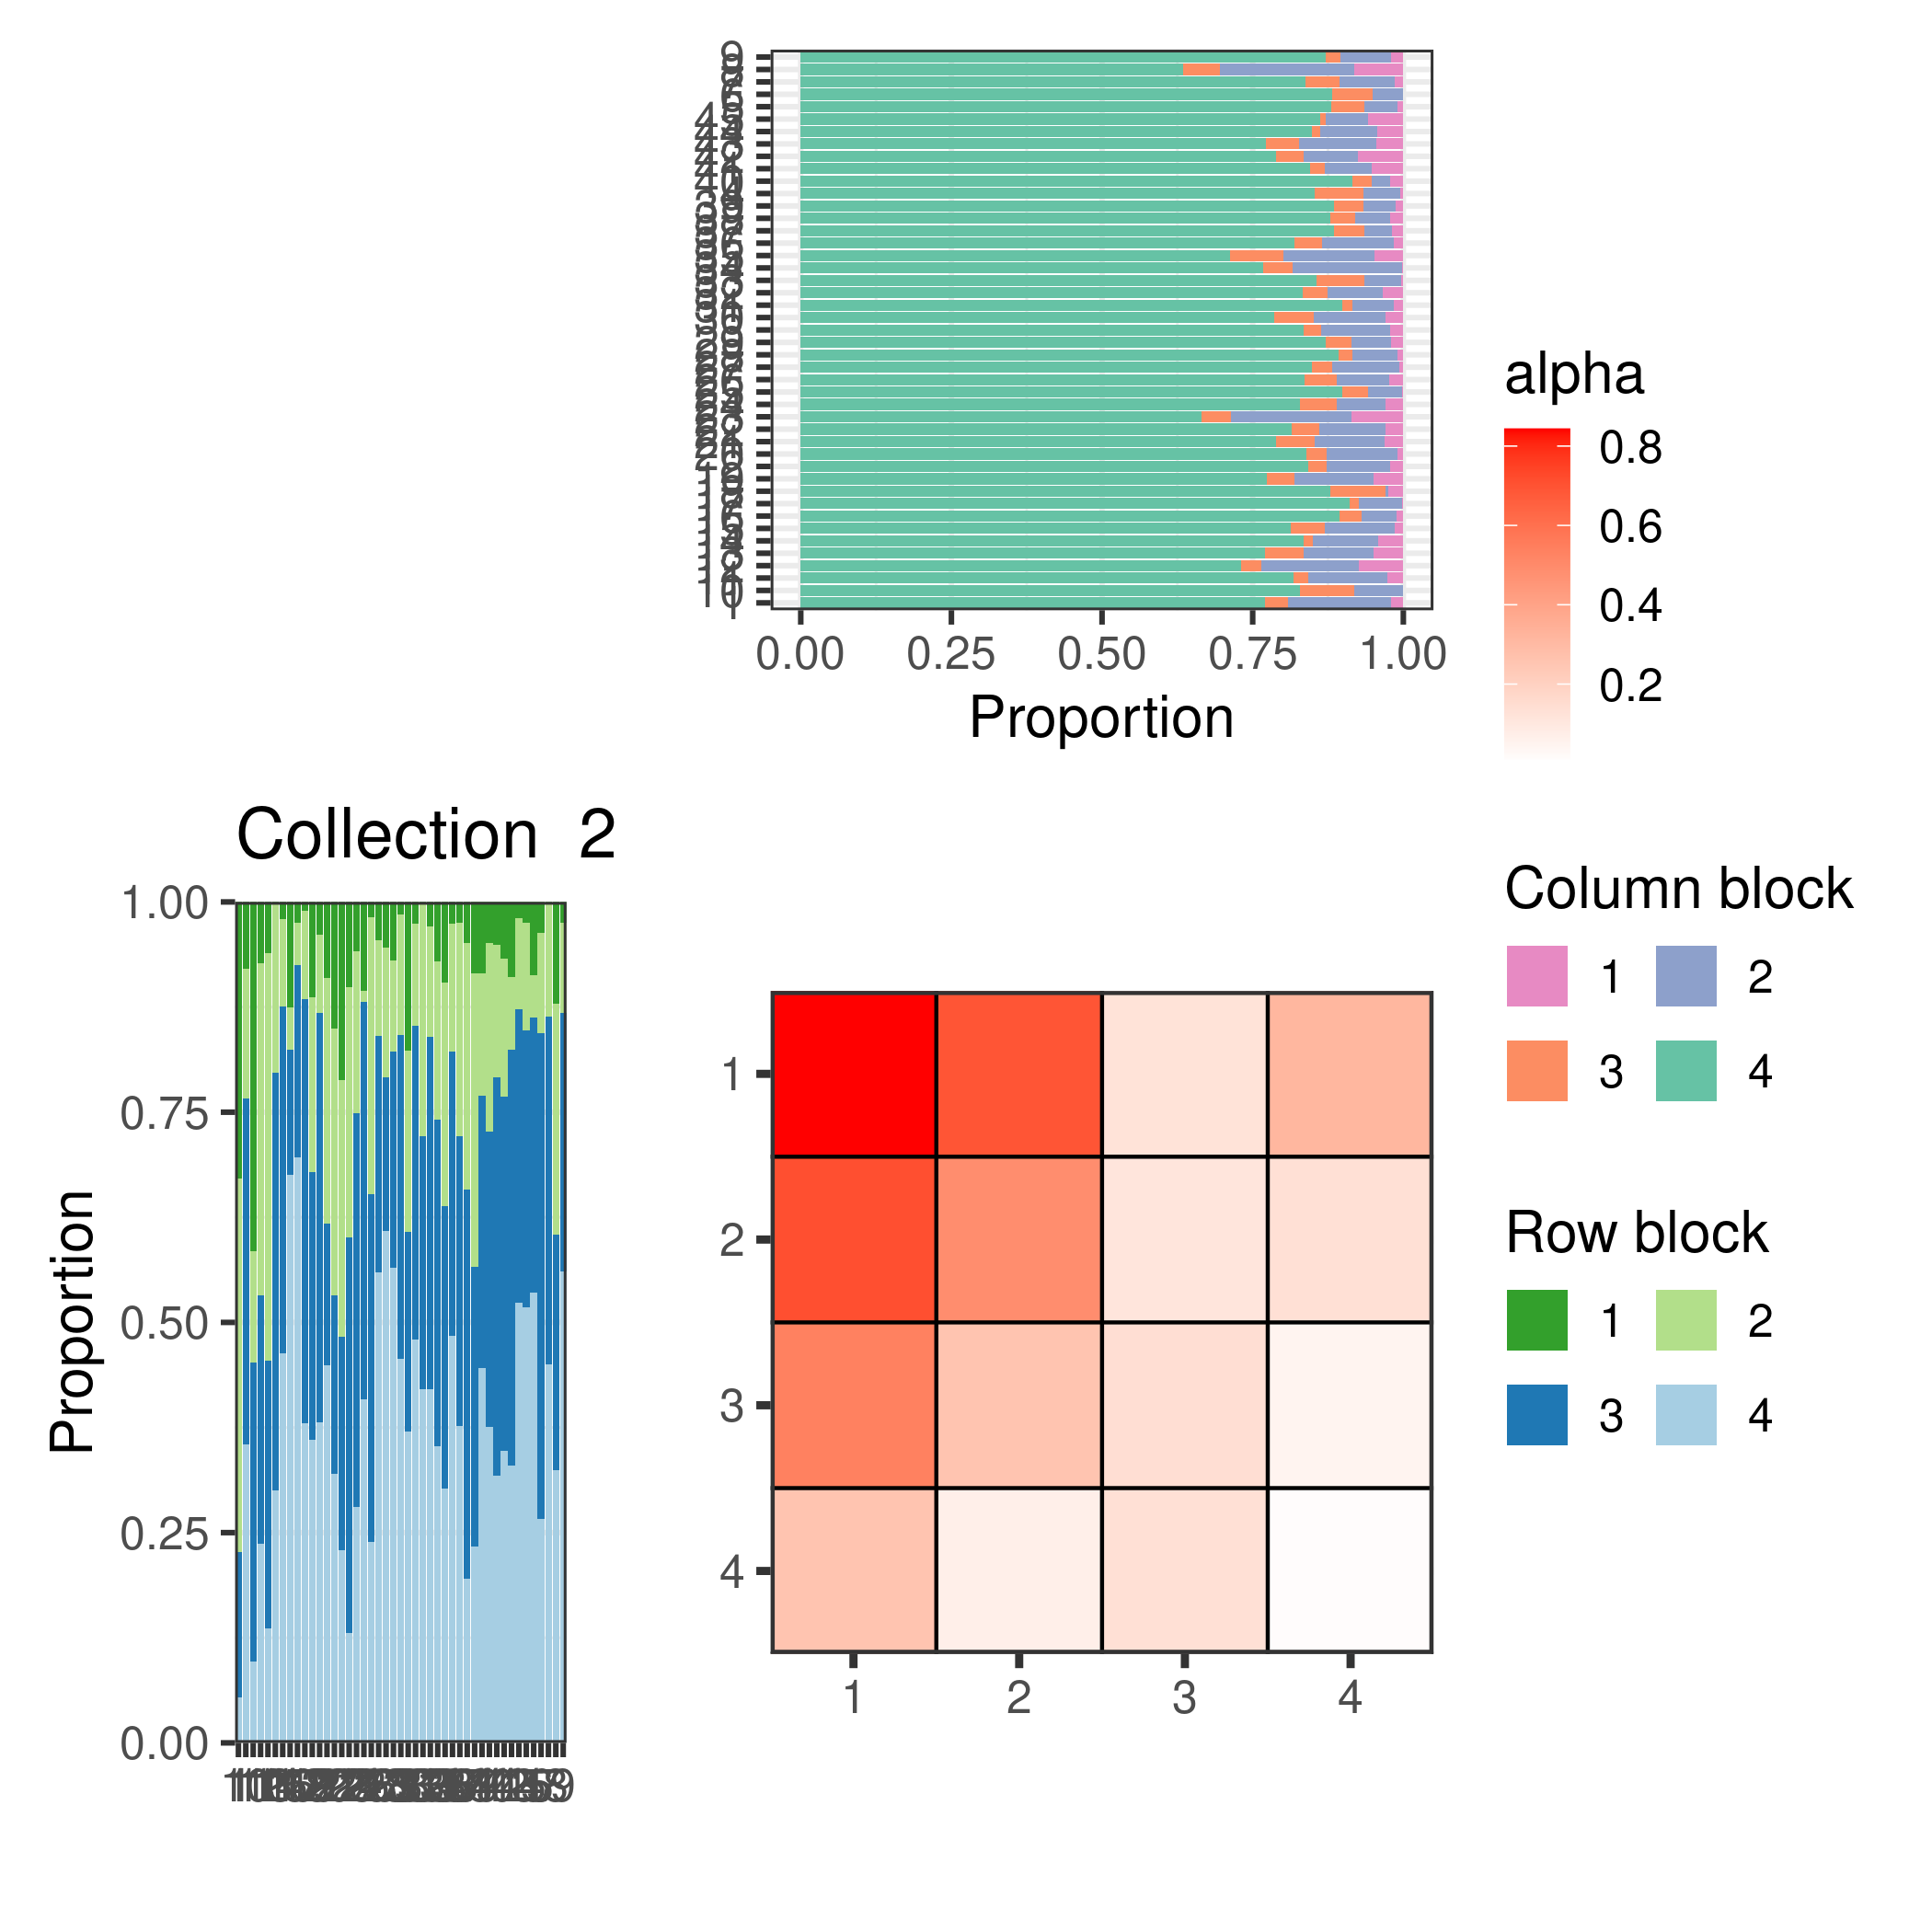
\includegraphics{./img/2859d1c94af6539cced6aee6ee6bf6d49498518d.png}\newline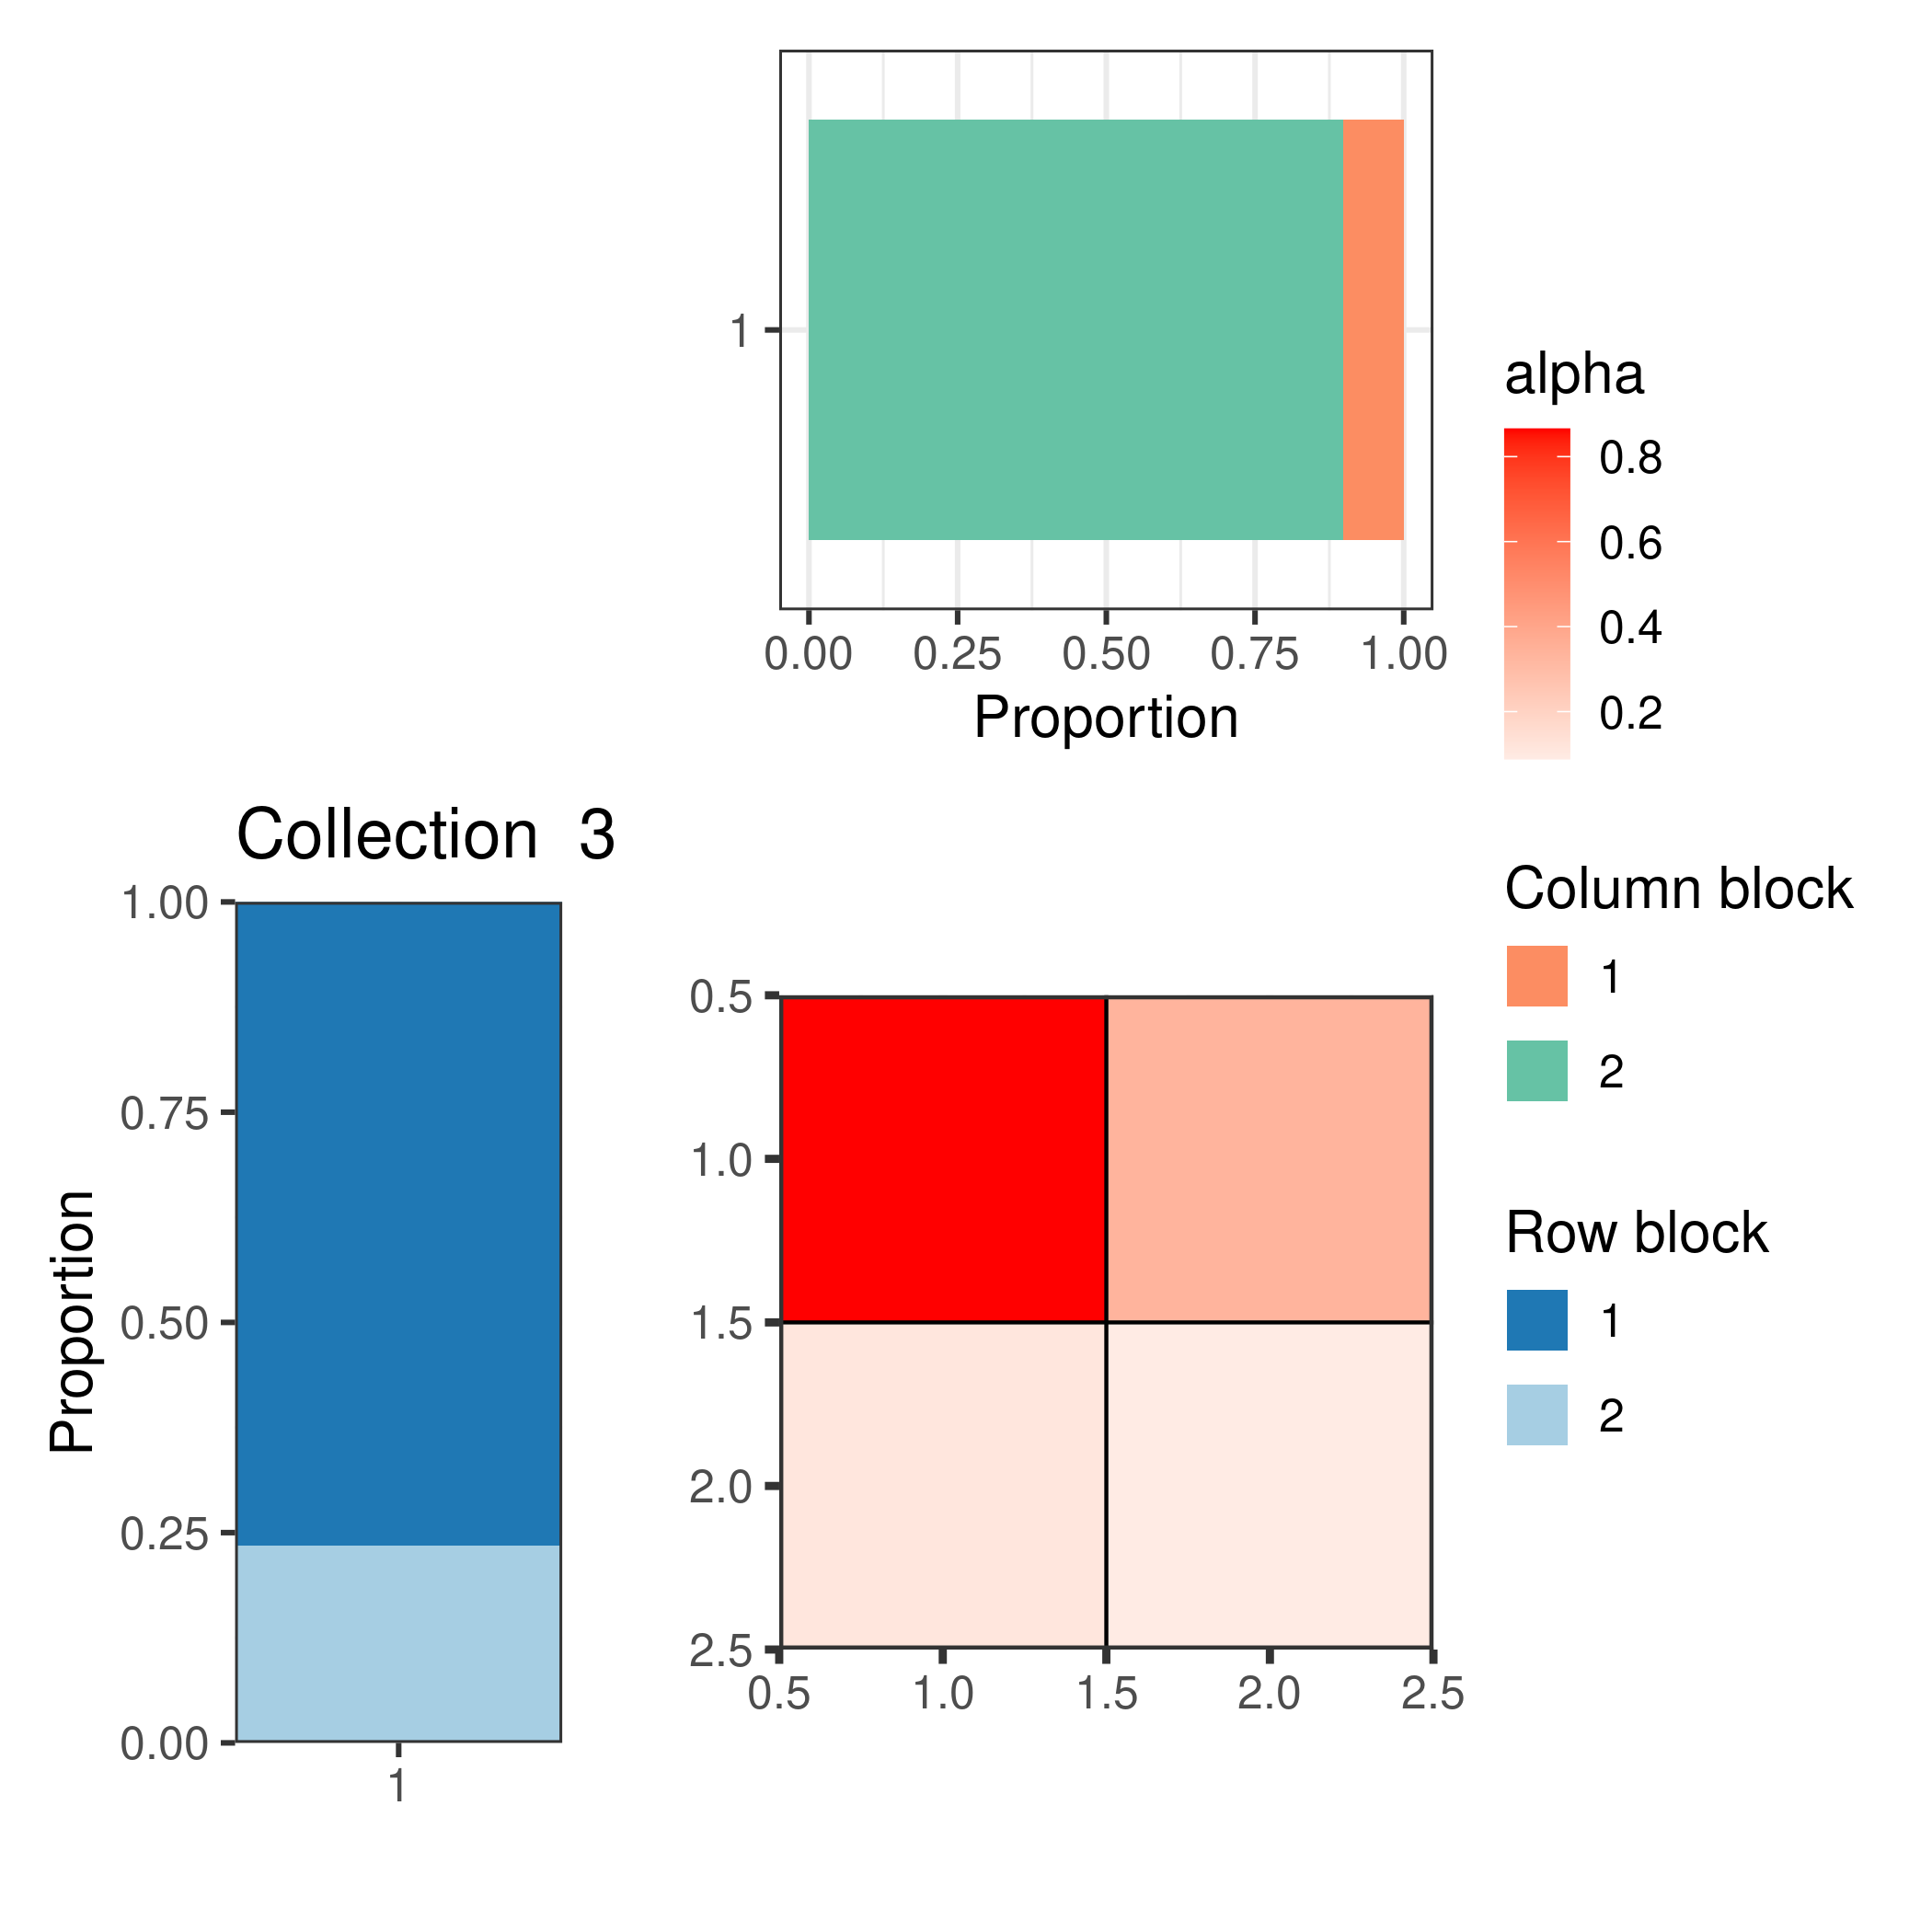
\includegraphics{./img/037bcbcbc85f8a9562f98706ad7766c4099516ef.png}\newline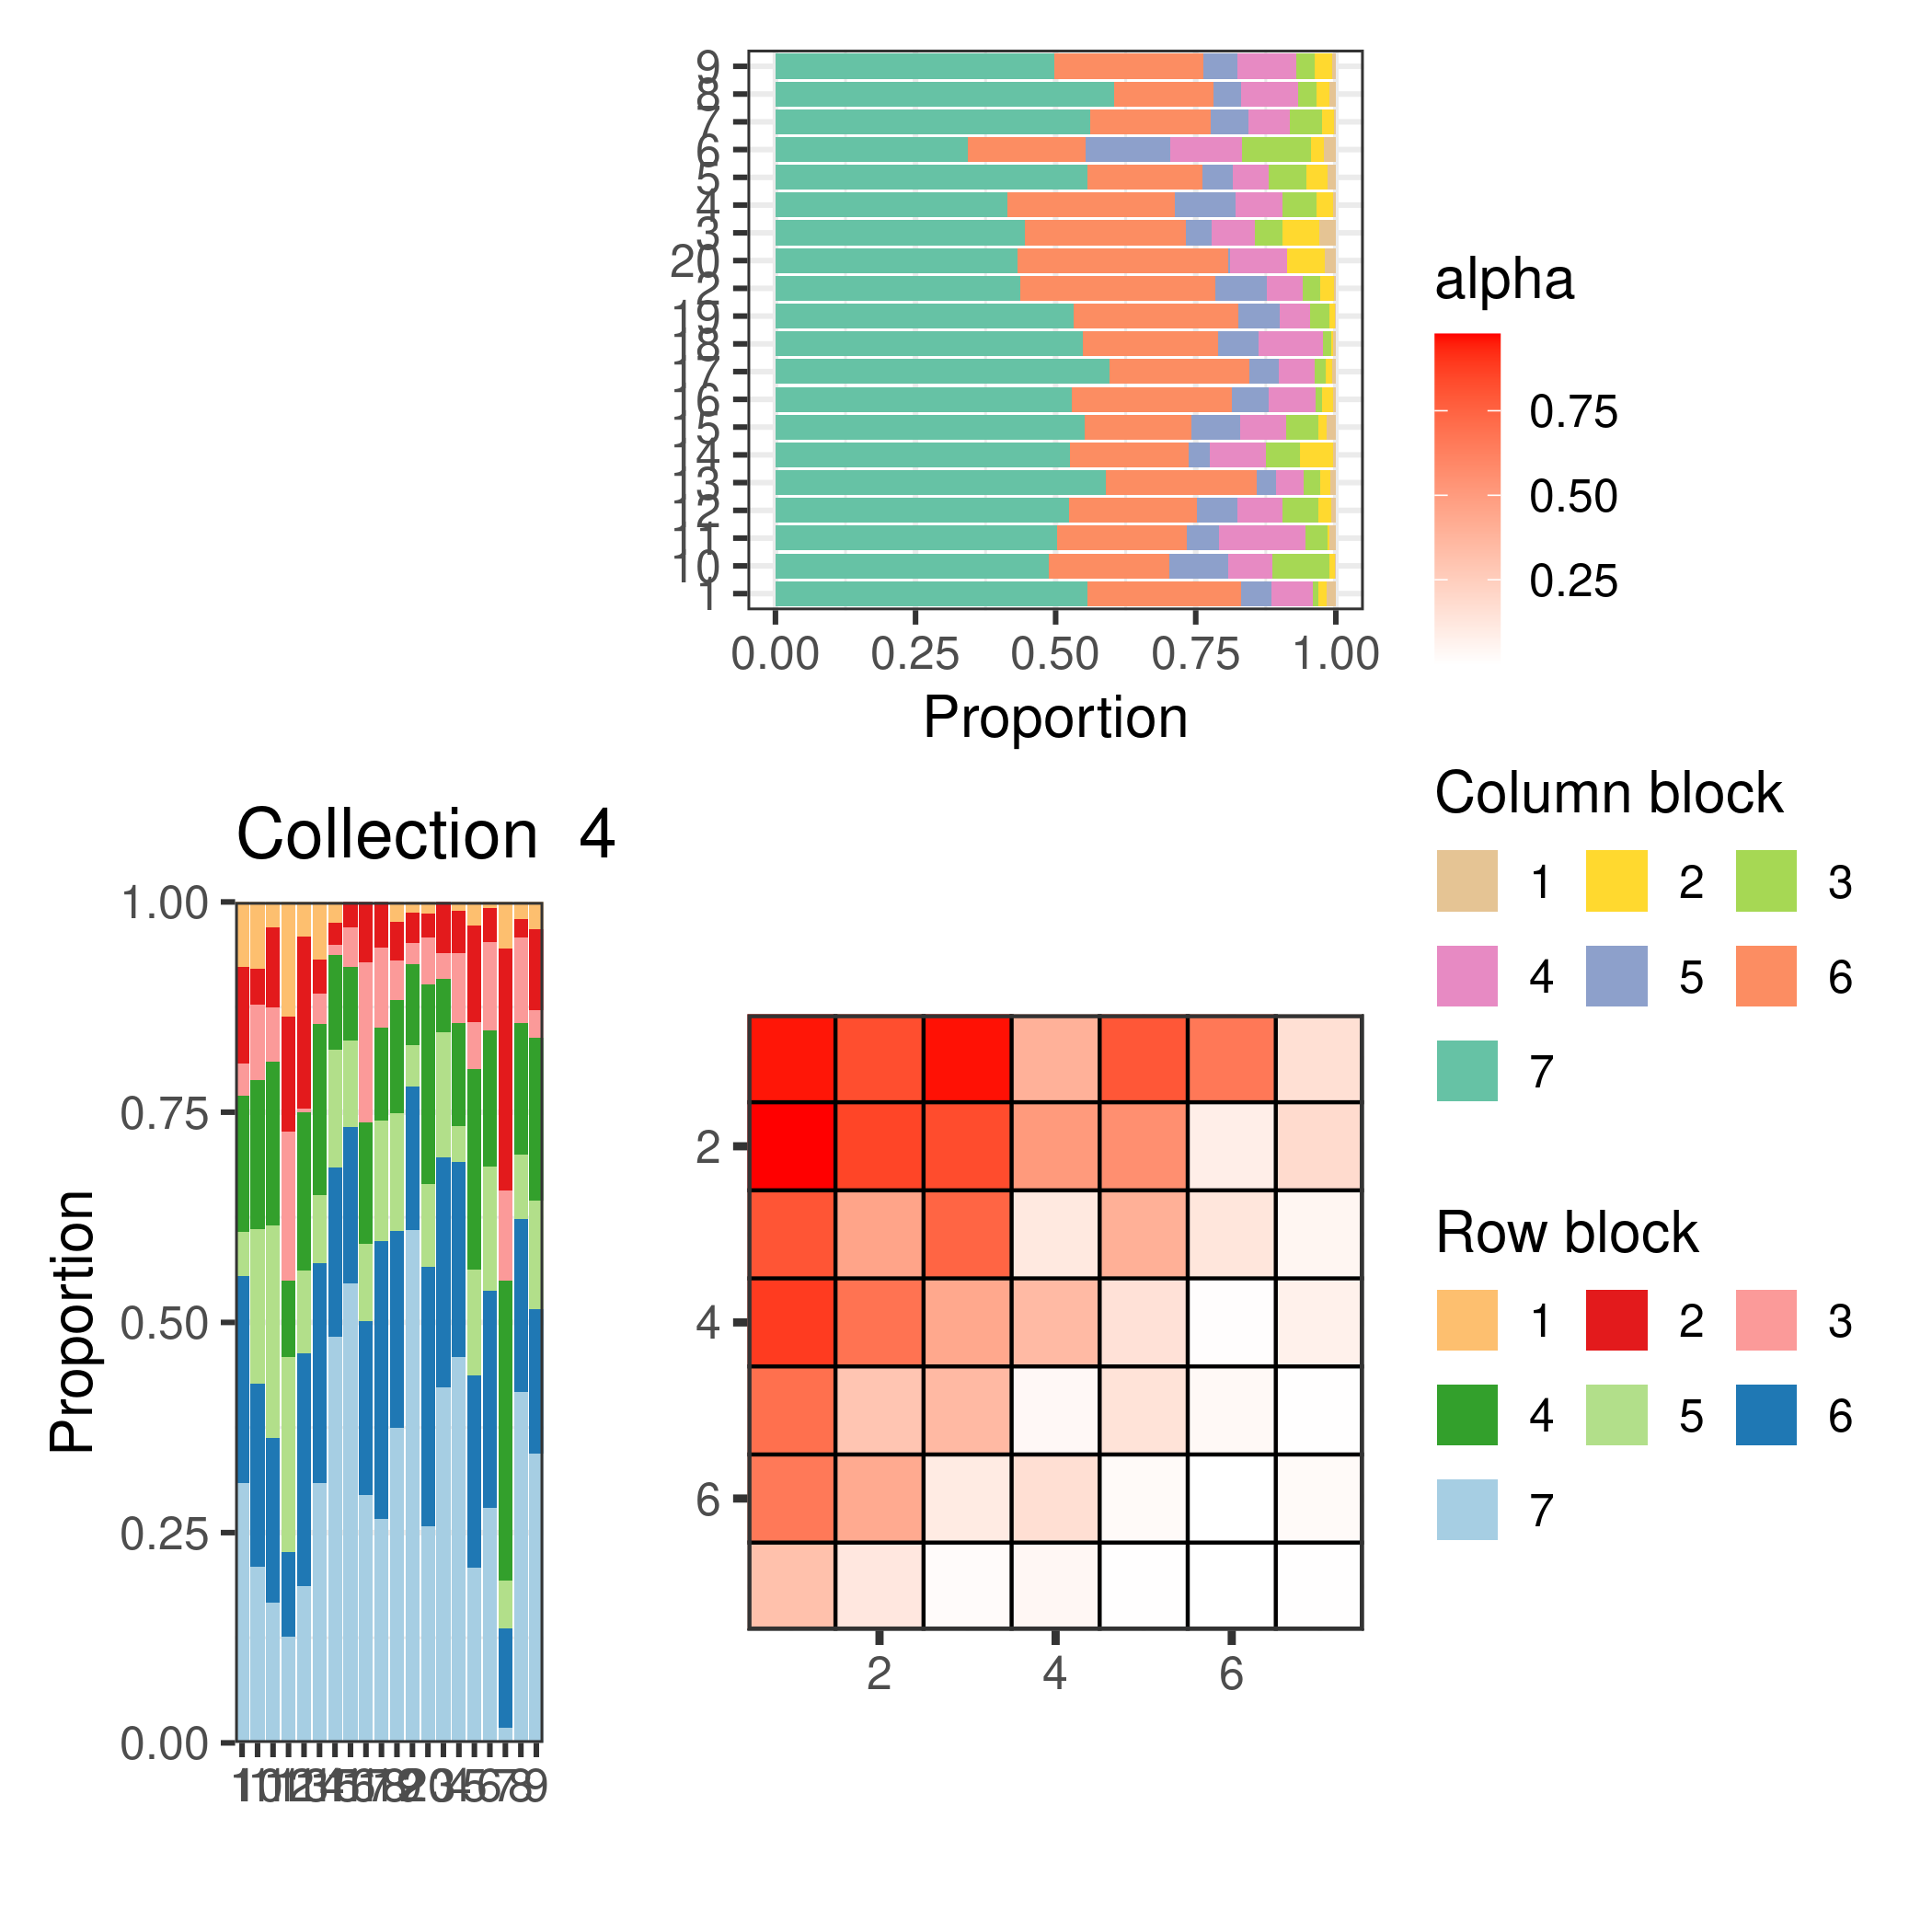
\includegraphics{./img/f730f05cb60a7cdc837102601660f03edd767a60.png}\newline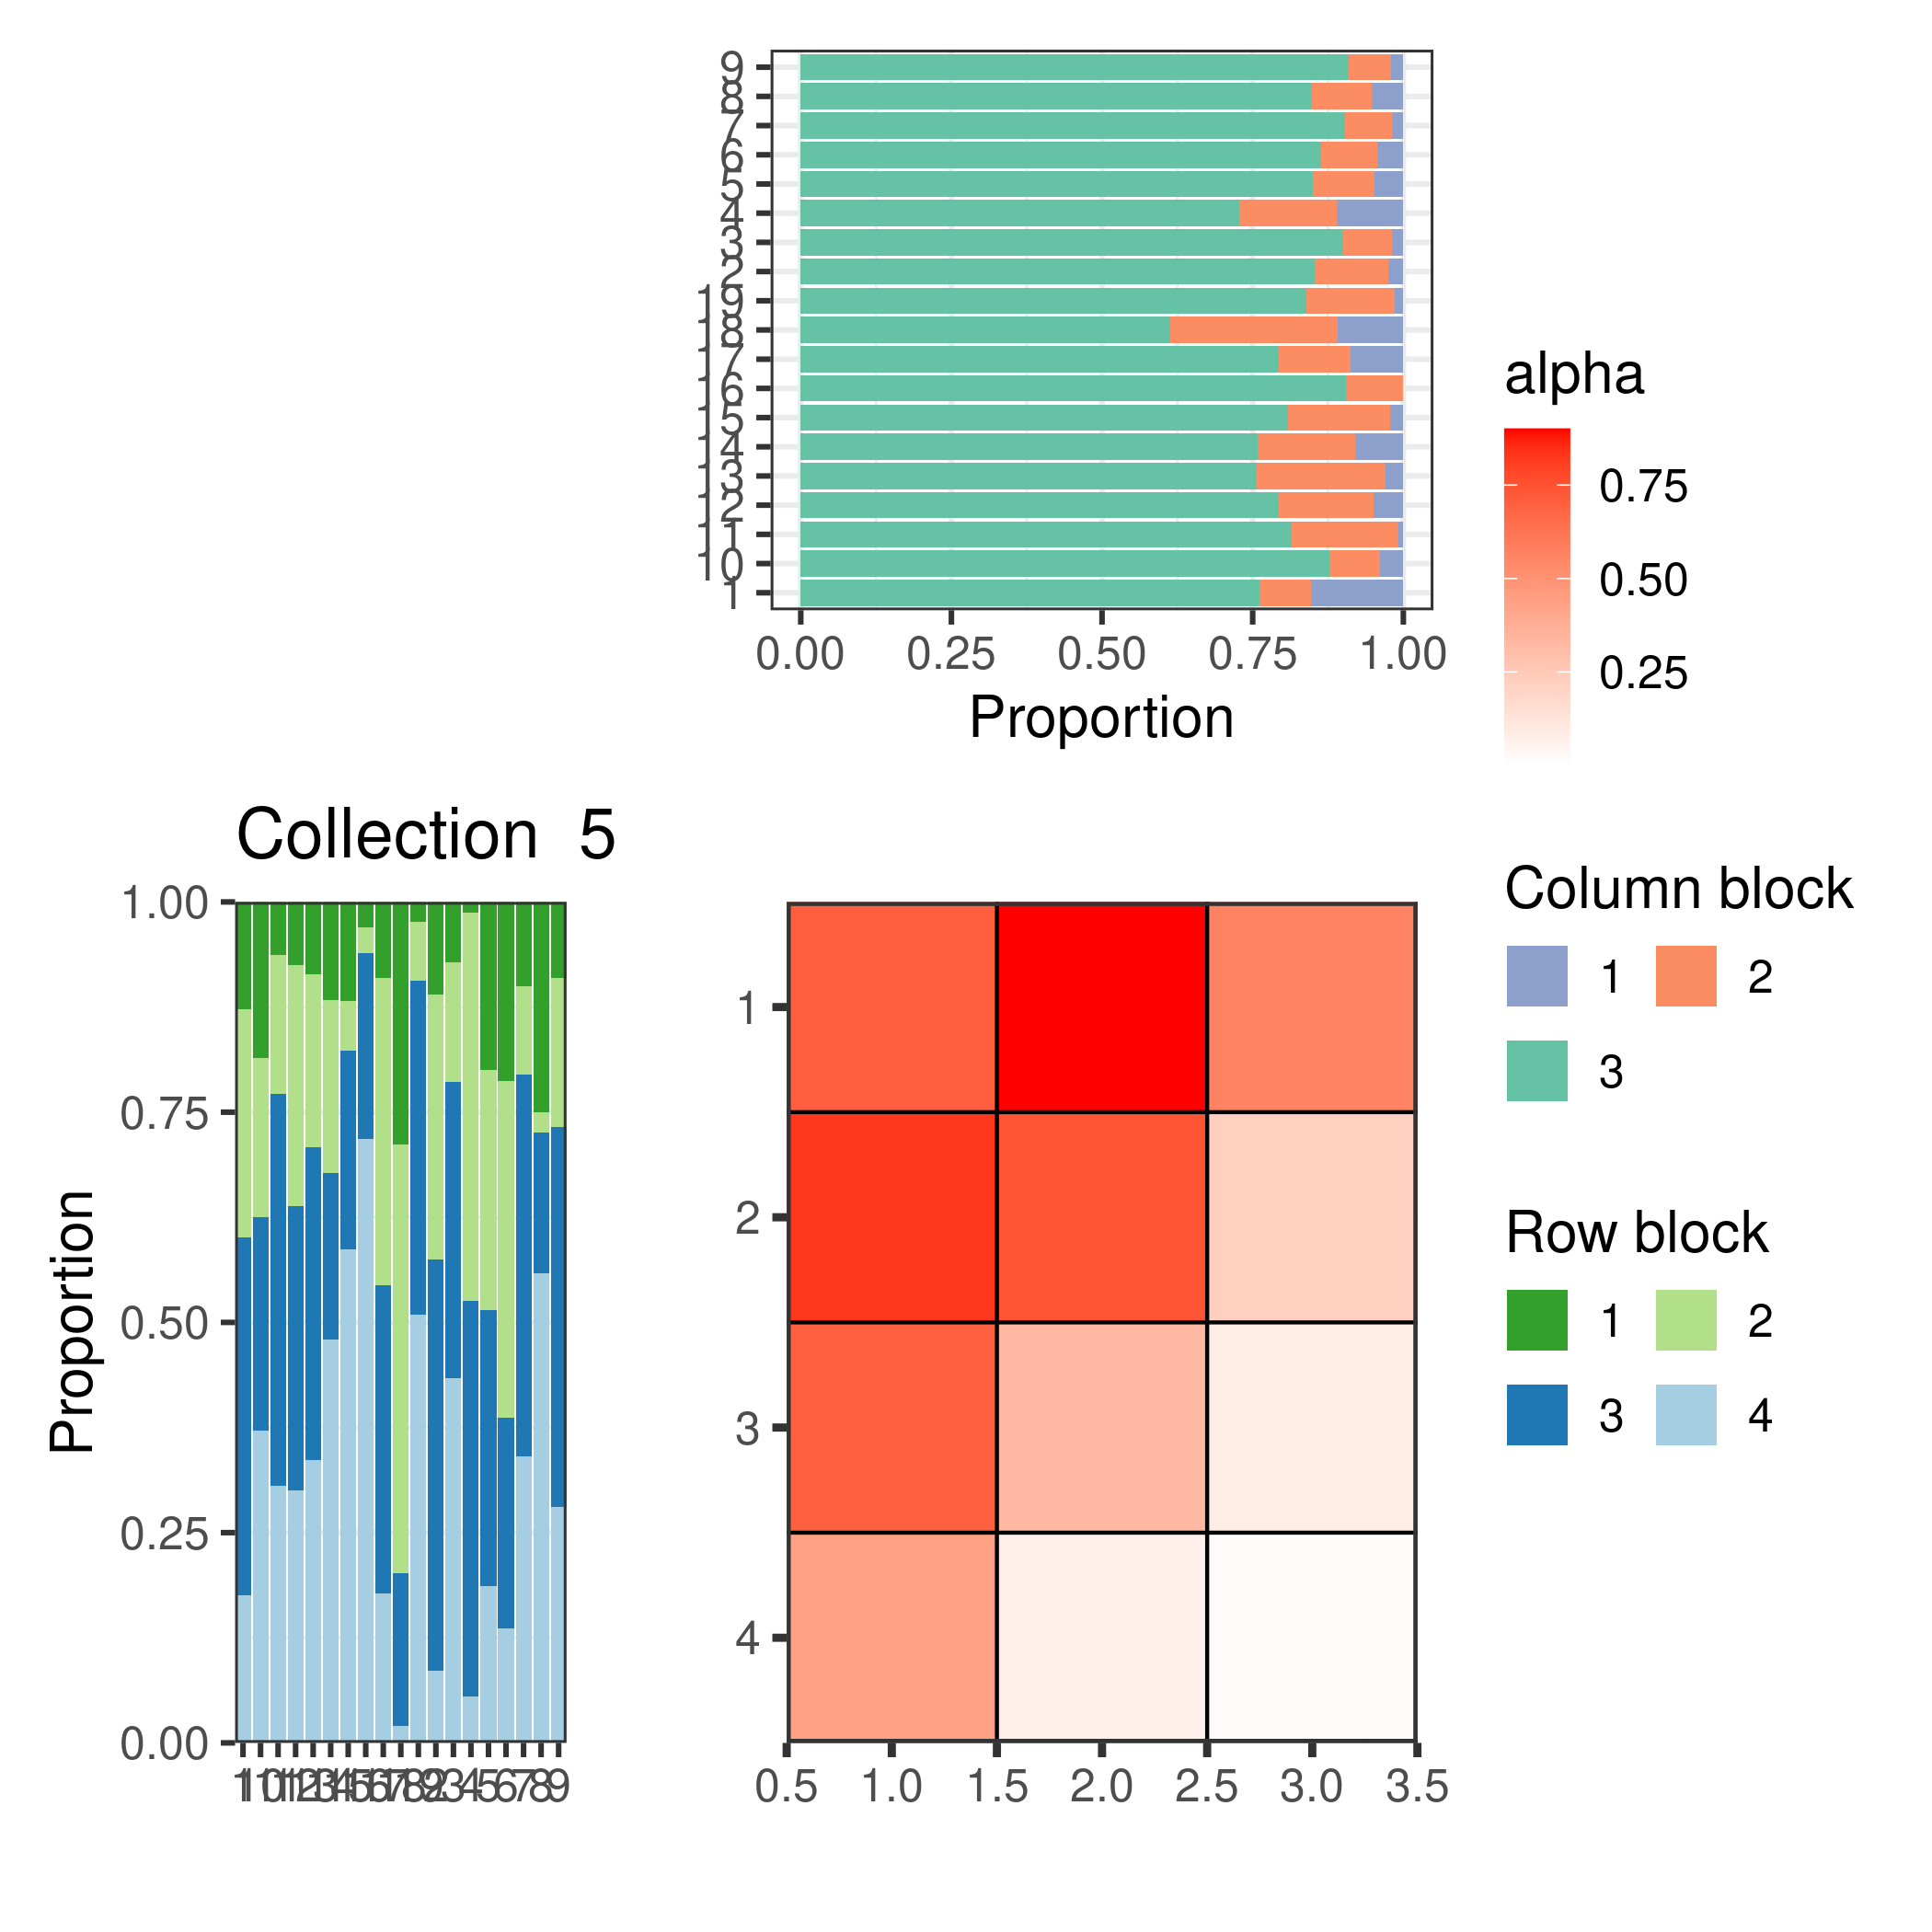
\includegraphics{./img/90d21c2459f68c2a6bc6cce93f9f1e10c3f0fef5.png}\newline

In all the obtained collections the structure is the classical nested
structure. As this is a well-known structure for plant-pollinator data
this tends to indicate that we are not going in a wrong direction.

The \nth{3} collection consists of only one network, indicating that for
this model, the small76 network was really different of all the others.
One reason might be that it's the oldest network and maybe the data
collection protocol is different.

\hypertarget{comparison-with-additional-information}{%
\subsection{Comparison with additional
information}\label{comparison-with-additional-information}}

Using supplementary information we obtain the following boxplots.

\begin{figure}
\centering
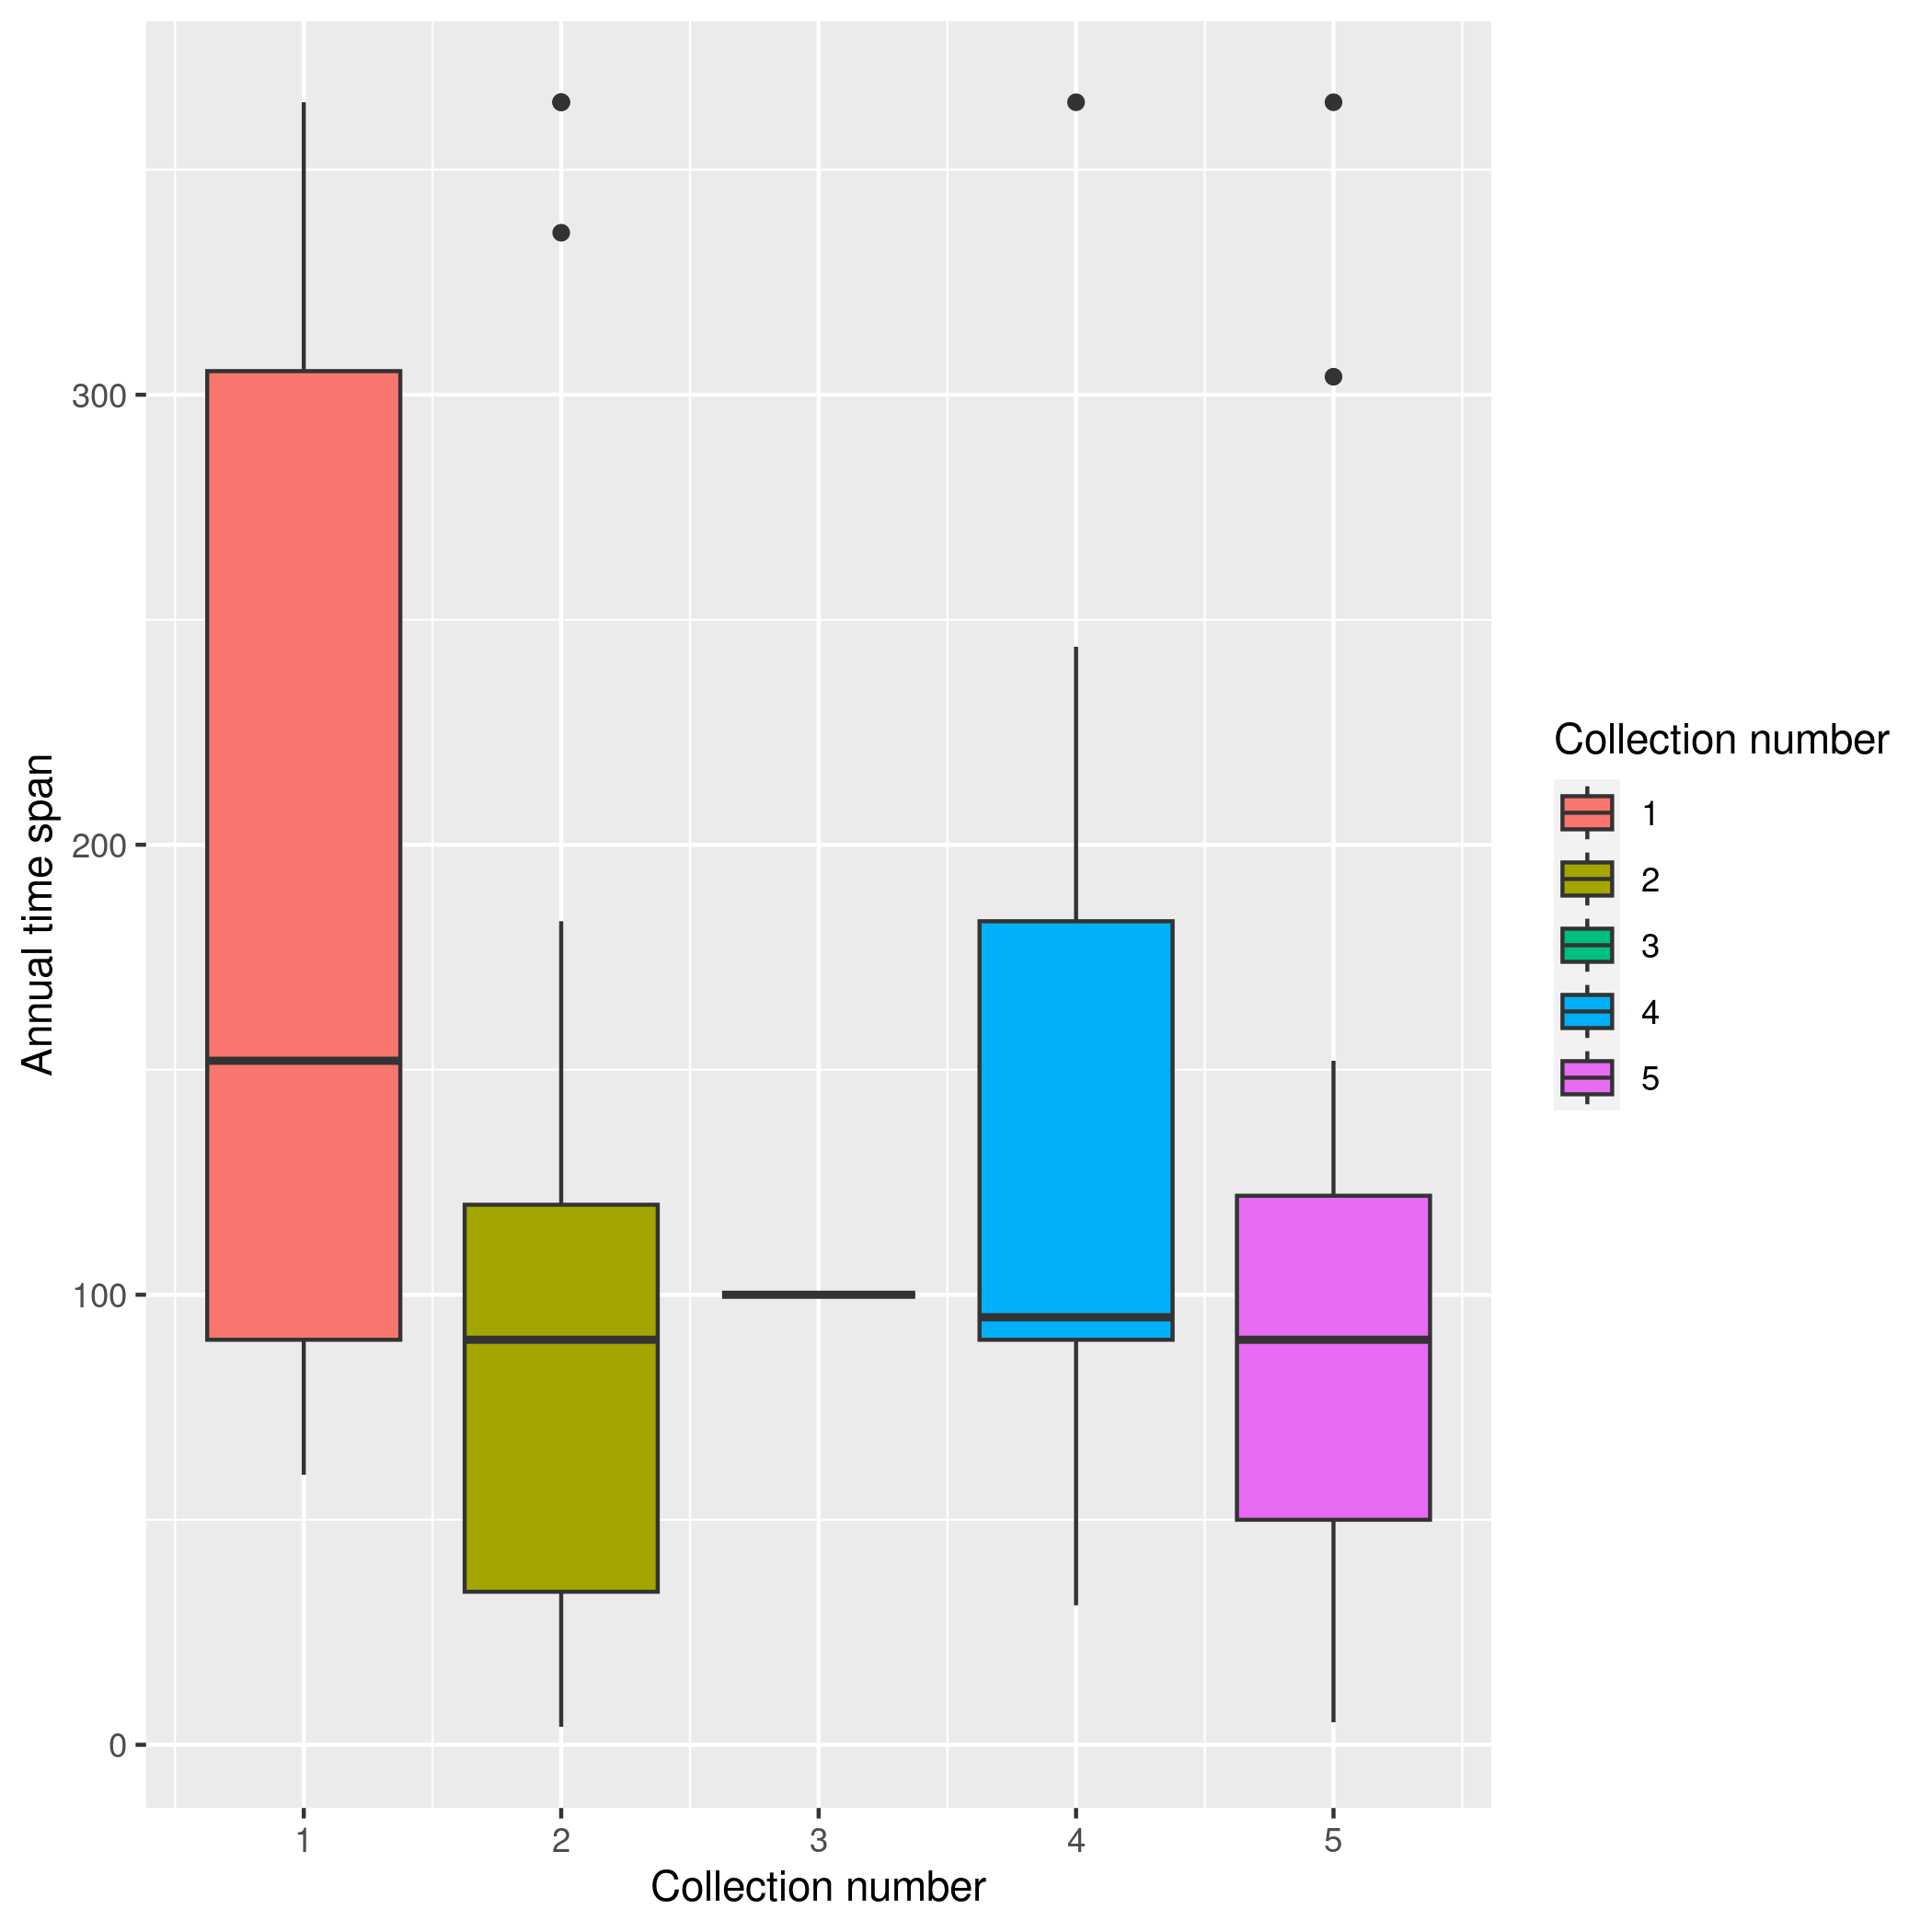
\includegraphics{./img/de77b630fb66744d3a3ed68e45be765532d1eb0f.png}
\caption{\label{fig:boxplot-annual-time-span}Boxplot of annual time span
in function of the collection number}
\end{figure}

The annual time span is the number of days the sampling period lasted.
So we can thus see in figure \ref{fig:boxplot-annual-time-span} that
collections 1 and 4 were sampled for a larger period of time than
collections 2 and 5. This could explain observed differences in the
structure detected : the ``checkerboard'' appearance of the alpha
matrices representations may represent interactions that only occurs at
a given period of time. Thus the shorter time period doesn't capture
such interactions.

\begin{figure}
\centering
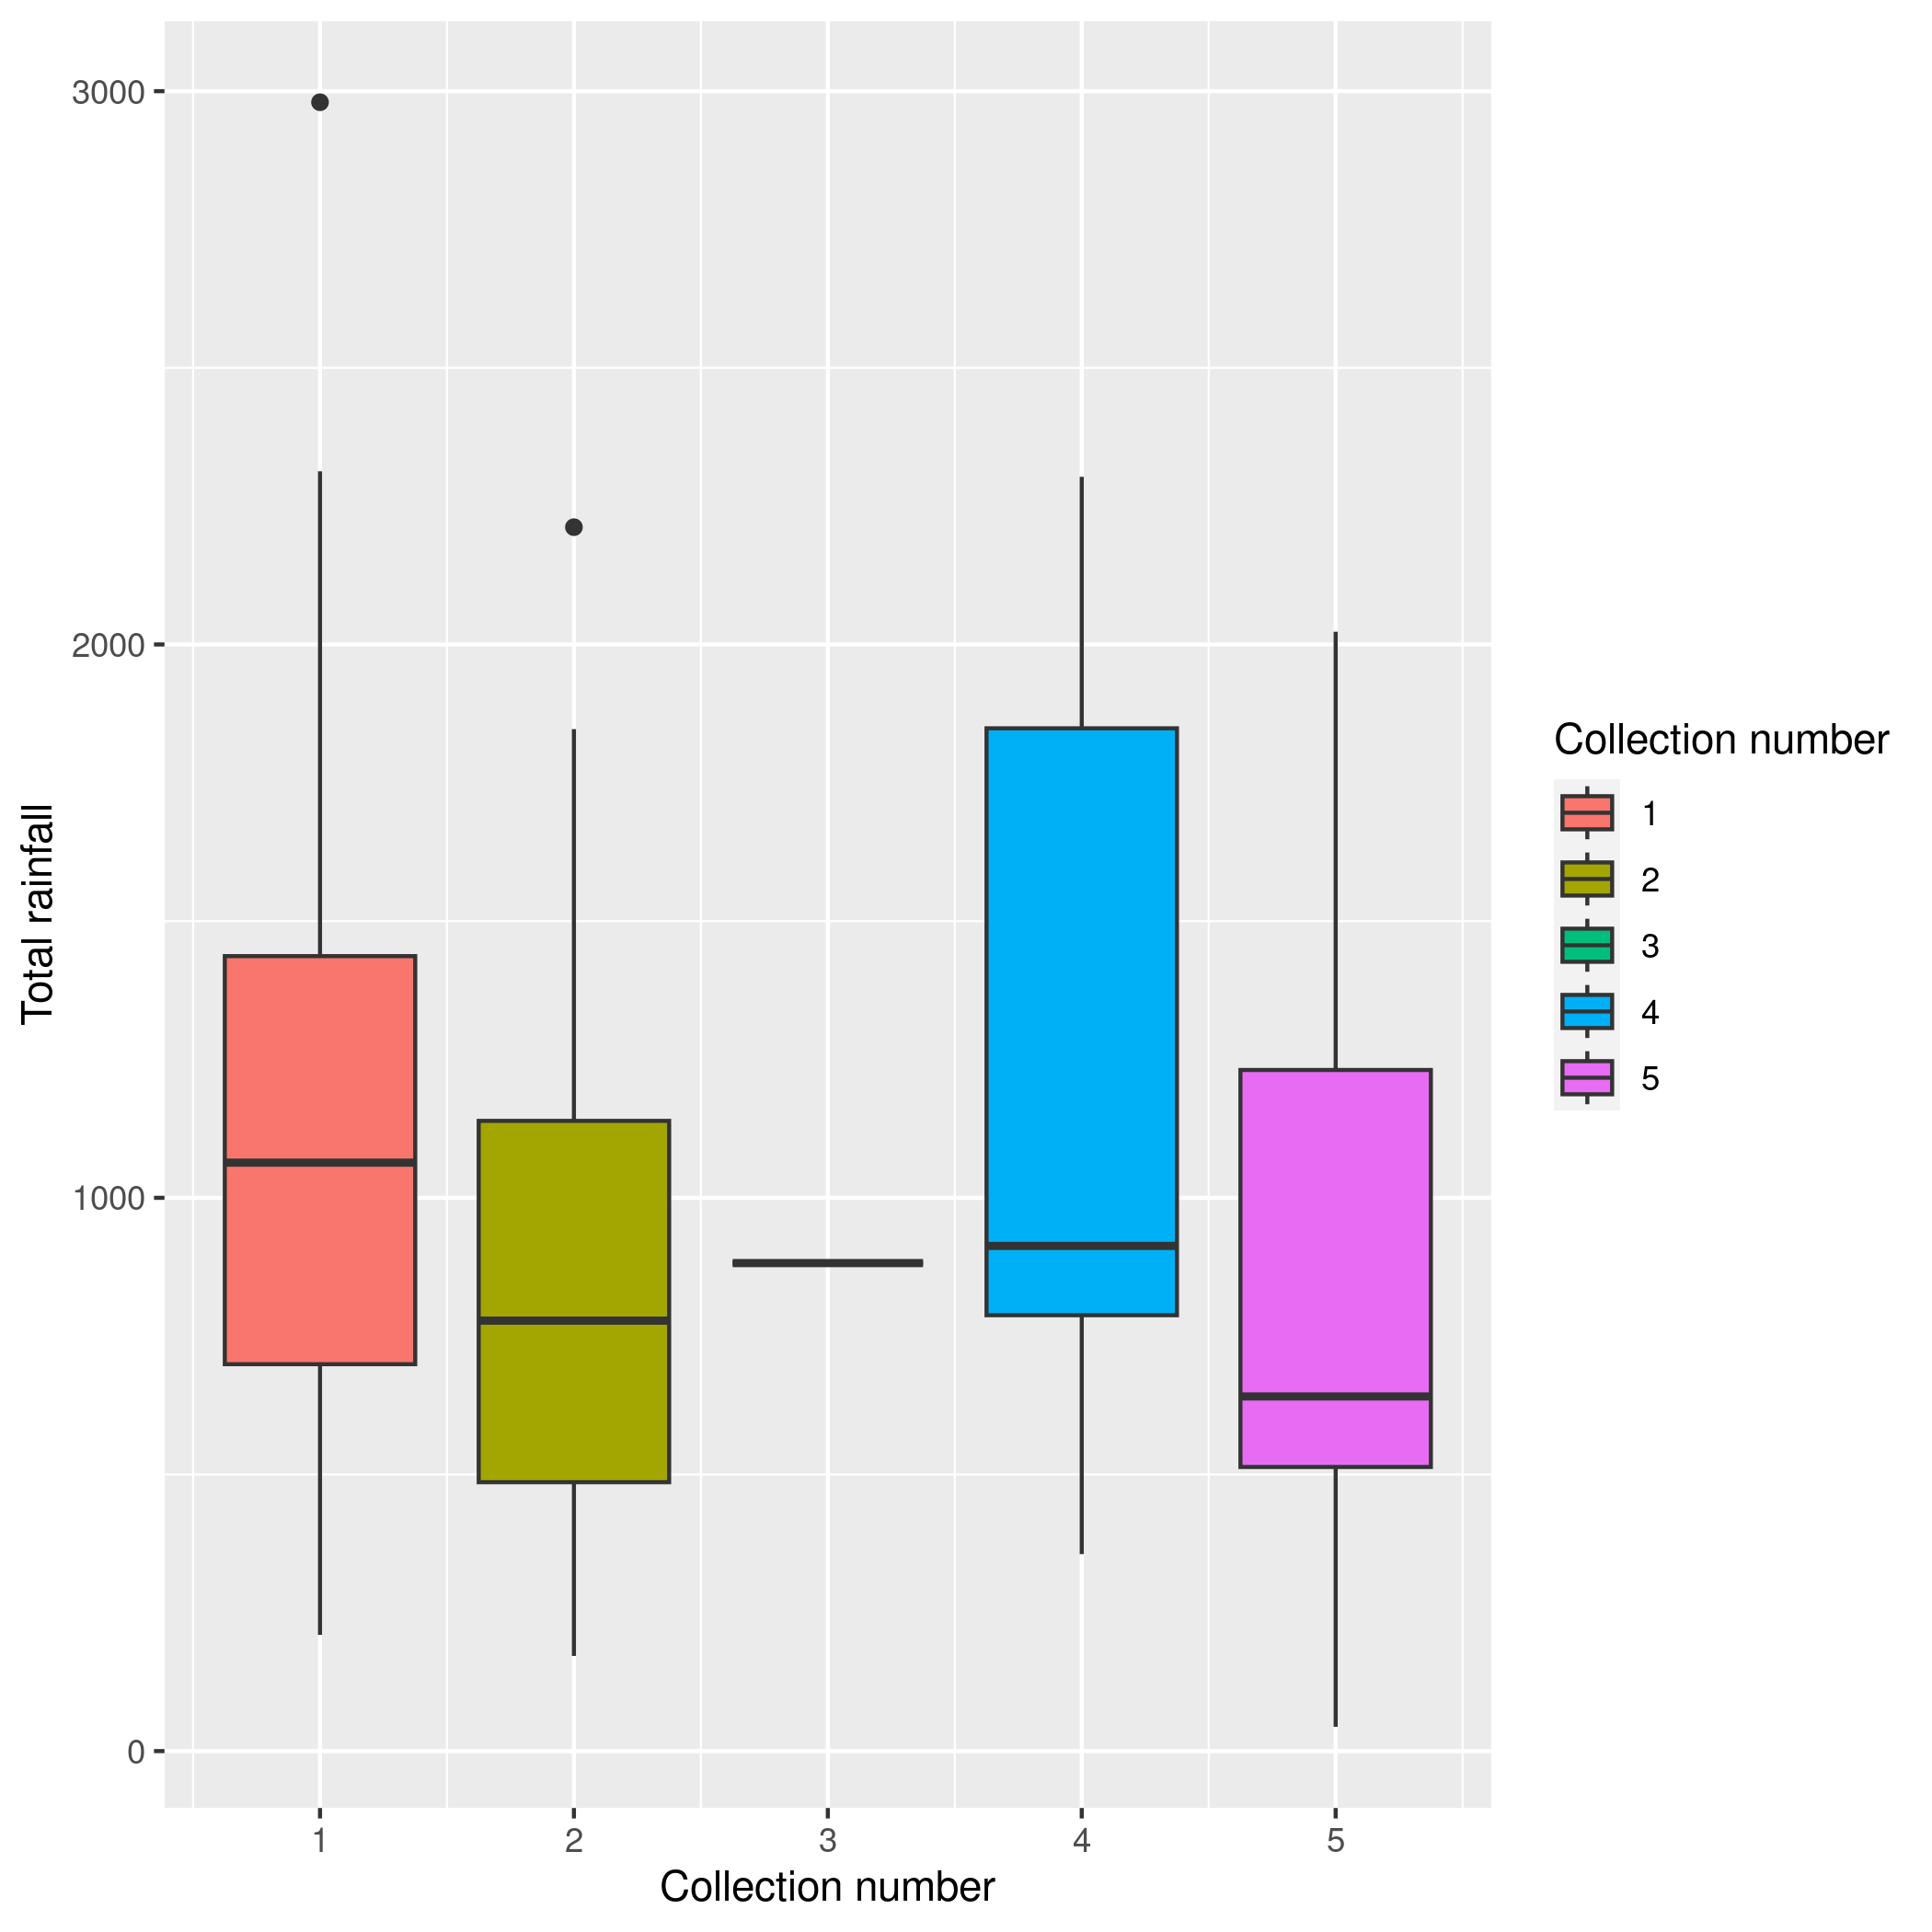
\includegraphics{./img/5bbc4b4b07c0e990a3ae2755165958ffbf517902.png}
\caption{\label{fig:boxplot-total-rainfall}Boxplot of total rainfall in
function of the collection number}
\end{figure}

There seems to be the same trend for the total rainfall.

\begin{figure}
\centering
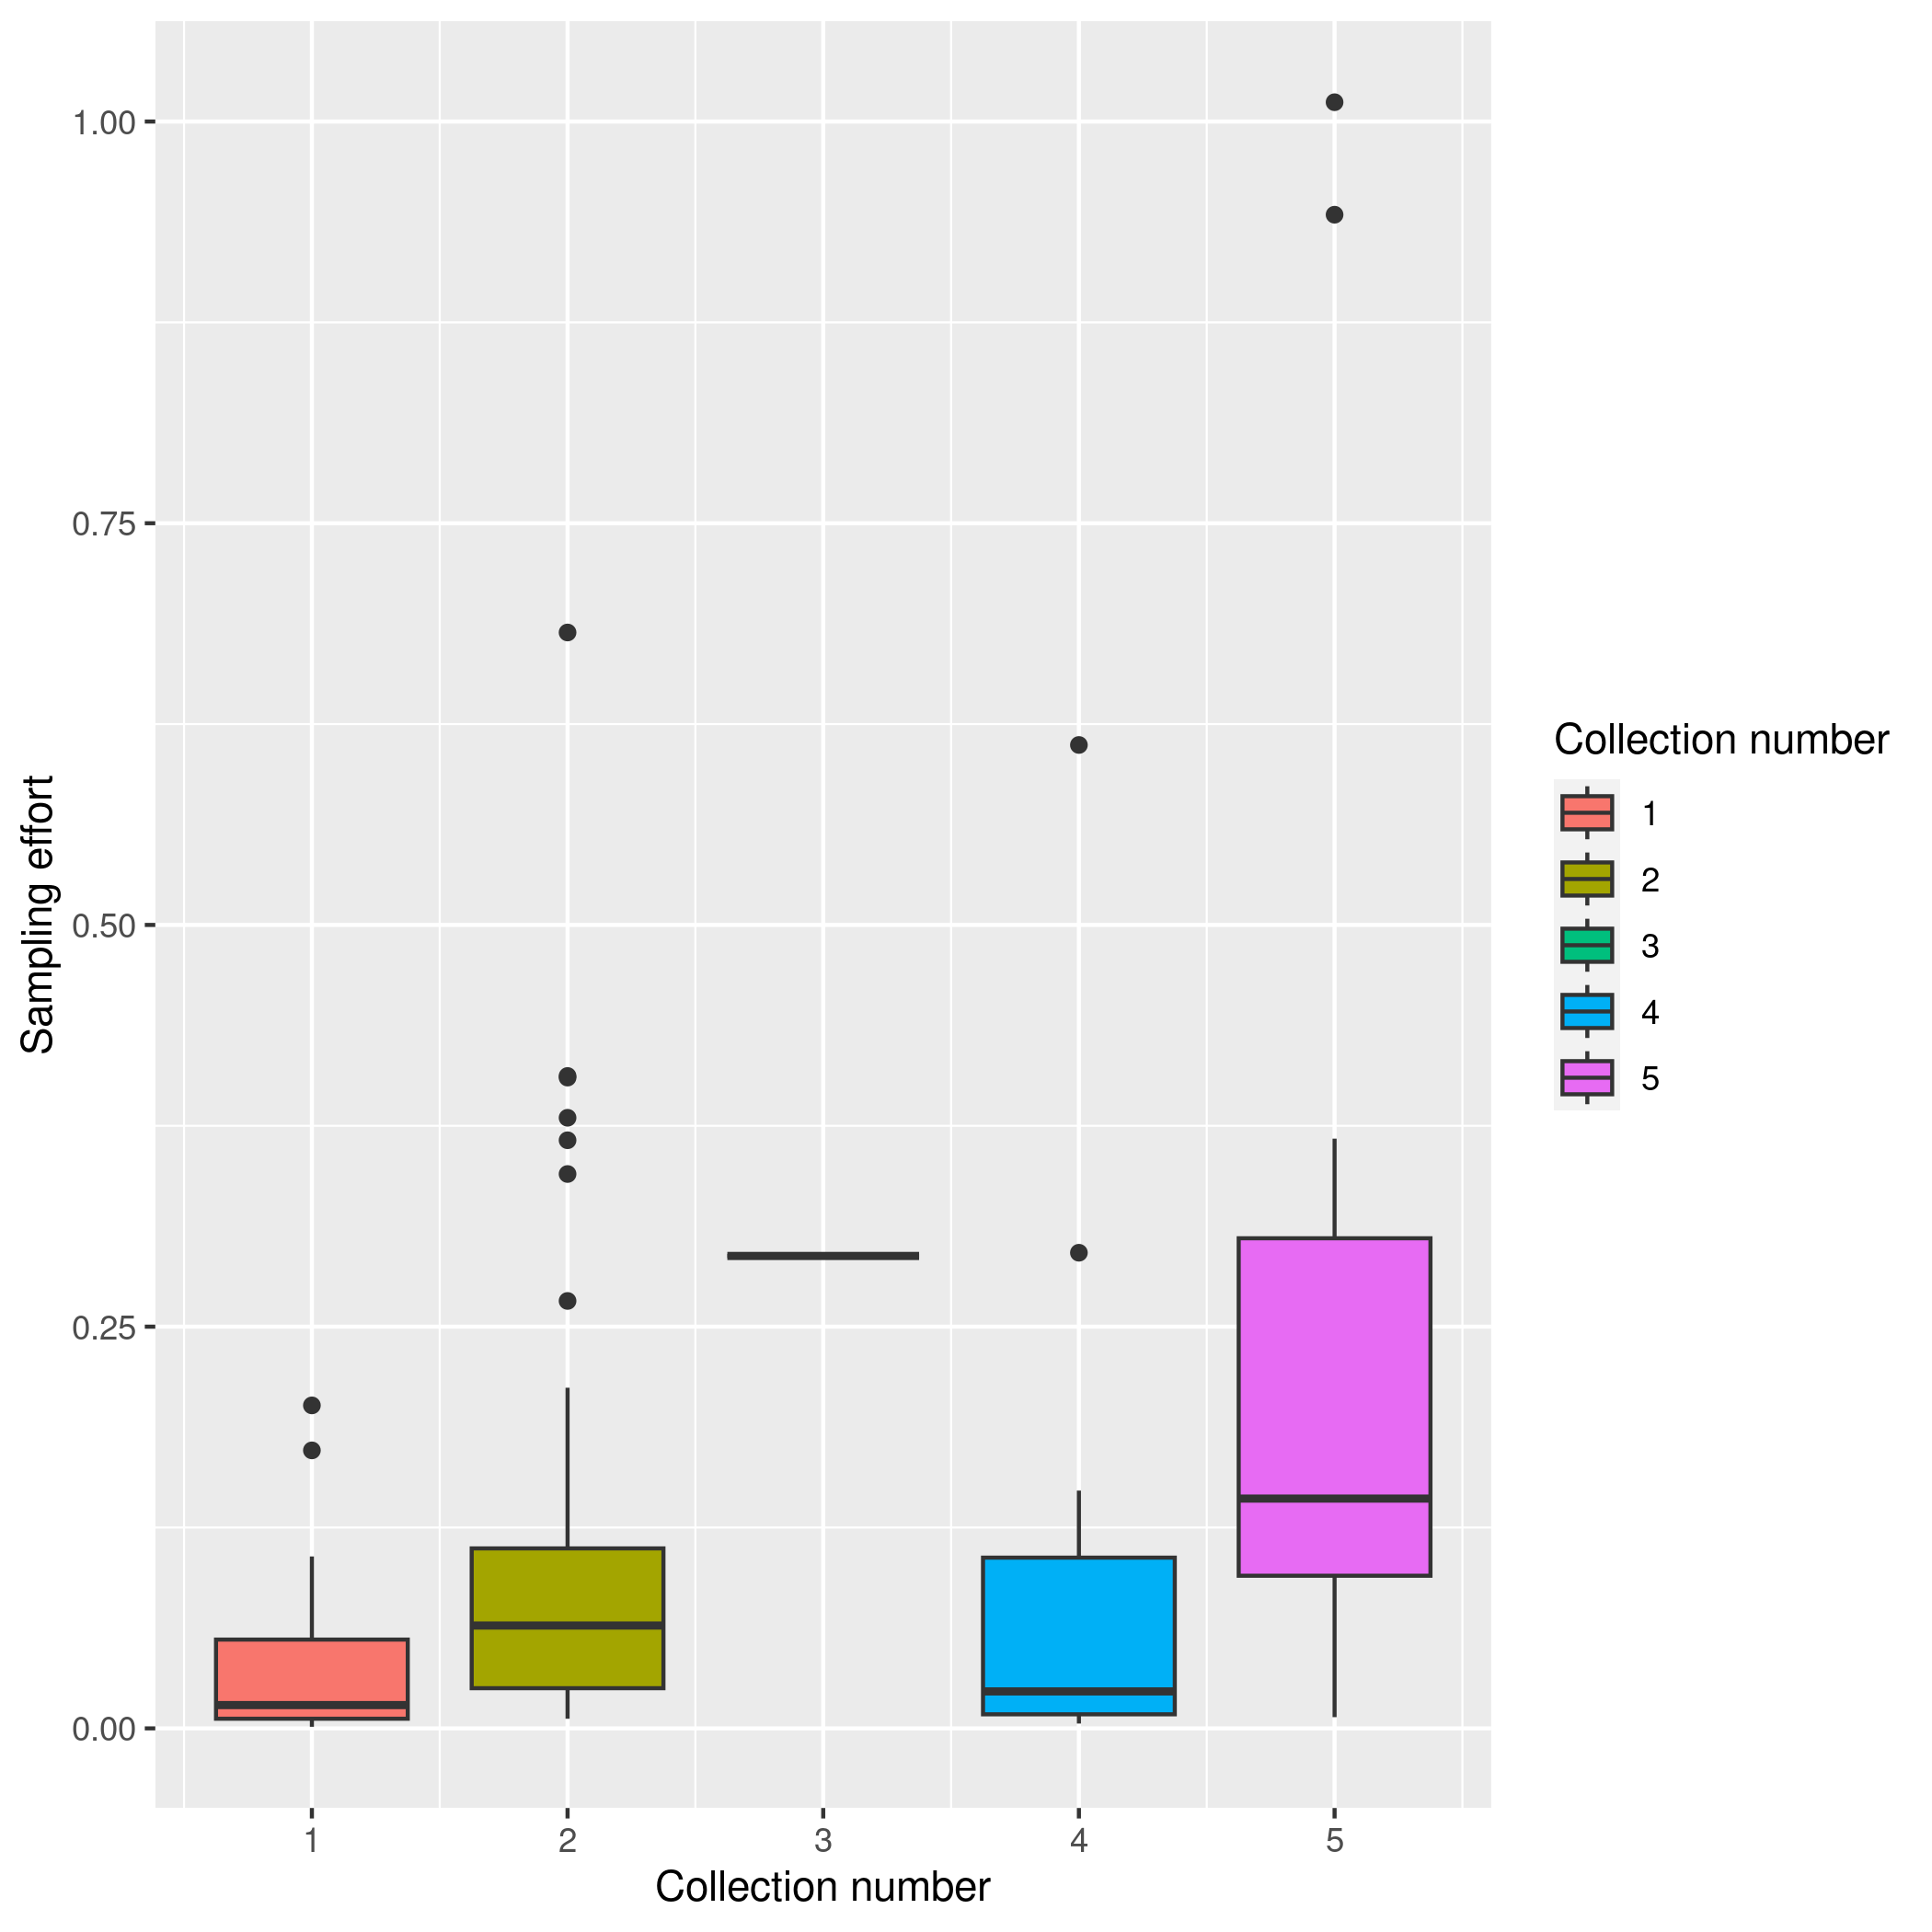
\includegraphics{./img/c75a33aa046b6f1bbcff45268346c4ec39067917.png}
\caption{\label{fig:boxplot-sampling-effort}Boxplot of the sampling
effort in function of the collection number}
\end{figure}

The sampling effort seems to be quite higher for collection 5 and a
little higher for collection 2. And collection 1 and 4 have the inverse
trend. The separation between collections 1,4 and 2,5 seems to still
hold. And the sampling effort is related to the sampling time that is
why it's higher for the collections that were sampled for a shorter time
period.
